%%%%%%%%%%%%%%%%%%%%%%%%%%%%%%%%%%%%%%%%%%%%%%%%%%%%%%%%%%%%%%%%%%
%%%%%%%%%%%%%%%%%%%%%%%%%%%%%%%%%%%%%%%%%%%%%%%%%%%%%%%%%%%%%%%%%%
%Packages
\documentclass[10pt, a4paper]{article}
\usepackage[UTF8]{ctex}
\usepackage[top=3cm, bottom=4cm, left=3.5cm, right=3.5cm]{geometry}
\usepackage{amsmath,amsthm,amsfonts,amssymb,amscd, fancyhdr, color, comment, graphicx, environ}
\usepackage{float}
\usepackage{mathrsfs}
\usepackage[math-style=ISO]{unicode-math}
\setmathfont{TeX Gyre Termes Math}
\usepackage{lastpage}
\usepackage[dvipsnames]{xcolor}
\usepackage[framemethod=TikZ]{mdframed}
\usepackage{enumerate}
\usepackage[shortlabels]{enumitem}
\usepackage{fancyhdr}
\usepackage{indentfirst}
\usepackage{listings}
\usepackage{sectsty}
\usepackage{thmtools}
\usepackage{shadethm}
\usepackage{hyperref}
\usepackage{CJKfntef}
\usepackage{setspace}
\hypersetup{
    colorlinks=true,
    linkcolor=blue,
    filecolor=magenta,      
    urlcolor=blue,
}
%%%%%%%%%%%%%%%%%%%%%%%%%%%%%%%%%%%%%%%%%%%%%%%%%%%%%%%%%%%%%%%%%%
%%%%%%%%%%%%%%%%%%%%%%%%%%%%%%%%%%%%%%%%%%%%%%%%%%%%%%%%%%%%%%%%%%
%Environment setup
\mdfsetup{skipabove=\topskip,skipbelow=\topskip}
\newrobustcmd\ExampleText{%
An \textit{inhomogeneous linear} differential equation has the form
\begin{align}
L[v ] = f,
\end{align}
where $L$ is a linear differential operator, $v$ is the dependent
variable, and $f$ is a given non−zero function of the independent
variables alone.
}
\mdfdefinestyle{theoremstyle}{%
linecolor=black,linewidth=1pt,%
frametitlerule=true,%
frametitlebackgroundcolor=gray!20,
innertopmargin=\topskip,
}
\mdtheorem[style=theoremstyle]{Problem}{作业题}
\newenvironment{Solution}{}

%%%%%%%%%%%%%%%%%%%%%%%%%%%%%%%%%%%%%%%%%%%%%%%%%%%%%%%%%%%%%%%%%%
%%%%%%%%%%%%%%%%%%%%%%%%%%%%%%%%%%%%%%%%%%%%%%%%%%%%%%%%%%%%%%%%%%
%Fill in the appropriate information below
\newcommand{\norm}[1]{\left\lVert#1\right\rVert}     
\newcommand\course{最优化方法}                         % <-- course name   
%\newcommand\hwnumber{1}                              % <-- homework number
\newcommand\Information{李邹/人工智能一班}          % <-- personal information
%%%%%%%%%%%%%%%%%%%%%%%%%%%%%%%%%%%%%%%%%%%%%%%%%%%%%%%%%%%%%%%%%%
%%%%%%%%%%%%%%%%%%%%%%%%%%%%%%%%%%%%%%%%%%%%%%%%%%%%%%%%%%%%%%%%%%
%Page setup
\pagestyle{fancy}
\headheight 35pt
\lhead{\today}
\rhead{
\includegraphics[width=2.5cm]{lzu-logo.png}}
\lfoot{}
\pagenumbering{arabic}
\cfoot{\small\thepage}
\rfoot{}
\headsep 1.2em
\renewcommand{\baselinestretch}{1.25}
%%%%%%%%%%%%%%%%%%%%%%%%%%%%%%%%%%%%%%%%%%%%%%%%%%%%%%%%%%%%%%%%%%
%%%%%%%%%%%%%%%%%%%%%%%%%%%%%%%%%%%%%%%%%%%%%%%%%%%%%%%%%%%%%%%%%%
%Add new commands here
\renewcommand{\labelenumi}{\alph{enumi})}
\newcommand{\Z}{\mathbb Z}
\newcommand{\R}{\mathbb R}
\newcommand{\Q}{\mathbb Q}
\newcommand{\NN}{\mathbb N}
\DeclareMathOperator{\Mod}{Mod} 
\renewcommand\lstlistingname{Algorithm}
\renewcommand\lstlistlistingname{Algorithms}
\def\lstlistingautorefname{Alg.}
%%%%%%%%%%%%%%%%%%%%%%%%%%%%%%%%%%%%%%%%%%%%%%%%%%%%%%%%%%%%%%%%%%
%%%%%%%%%%%%%%%%%%%%%%%%%%%%%%%%%%%%%%%%%%%%%%%%%%%%%%%%%%%%%%%%%%
%Begin now!



\begin{document}

\begin{titlepage}
    \begin{center}
        \vspace*{3.5cm}
            
        \Huge
        \textbf{作业8}
            
        \vspace{2cm}
        \LARGE
        李邹
            
        \vspace{0.1cm}
        \Large
        人工智能一班(2020级)                      % <-- author
        
            
        \vfill
        
        \course \ 课程作业
            
        \vspace{1cm}
            
        
\includegraphics[width=0.4\textwidth]{lzu-logo.png}
        \\
        
        \Large
        
        \today
            
    \end{center}
\end{titlepage}

%%%%%%%%%%%%%%%%%%%%%%%%%%%%%%%%%%%%%%%%%%%%%%%%%%%%%%%%%%%%%%%%%%
%%%%%%%%%%%%%%%%%%%%%%%%%%%%%%%%%%%%%%%%%%%%%%%%%%%%%%%%%%%%%%%%%%
%Start the assignment now

%%%%%%%%%%%%%%%%%%%%%%%%%%%%%%%%%%%%%%%%%%%%%%%%%%%%%%%%%%%%%%%%%%
%New problem
\newpage
\begin{Problem}
    考虑优化问题
    $$
    \begin{array}{ll}
    \operatorname{minimize} & f_{0}\left(x_{1}, x_{2}\right) \\
    \text {subject to} & 2 x_{1}+x_{2} \geq 1 \\
    & x_{1}+3 x_{2} \geq 1 \\
    & x_{1} \geq 0, \quad x_{2} \geq 0 .
    \end{array}
    $$
    对其可行集进行概述。对下面的每个目标函数,给出最优集和最优值。
    \begin{enumerate}[(a)]
    \item $f_{0}\left(x_{1}, x_{2}\right)=x_{1}+x_{2}$.
    \item $f_{0}\left(x_{1}, x_{2}\right)=-x_{1}-x_{2}$.
    \item $f_{0}\left(x_{1}, x_{2}\right)=x_{1}$.
    \item $f_{0}\left(x_{1}, x_{2}\right)=\max \left\{x_{1}, x_{2}\right\}$.
    \item $f_{0}\left(x_{1}, x_{2}\right)=x_{1}^{2}+9 x_{2}^{2}$.
    \end{enumerate}
\end{Problem}
    
\begin{Solution}
\textbf{解答}
\end{Solution}
%Complete the assignment now
由约束条件,可作出可行集如图1所示的多面体。

其中各顶点为$ (0, +∞), (0, 1), (\frac{2}{5}, \frac{1}{5}), (1, 0),(+∞, 0)$.
\begin{figure}[H]
    \centering
    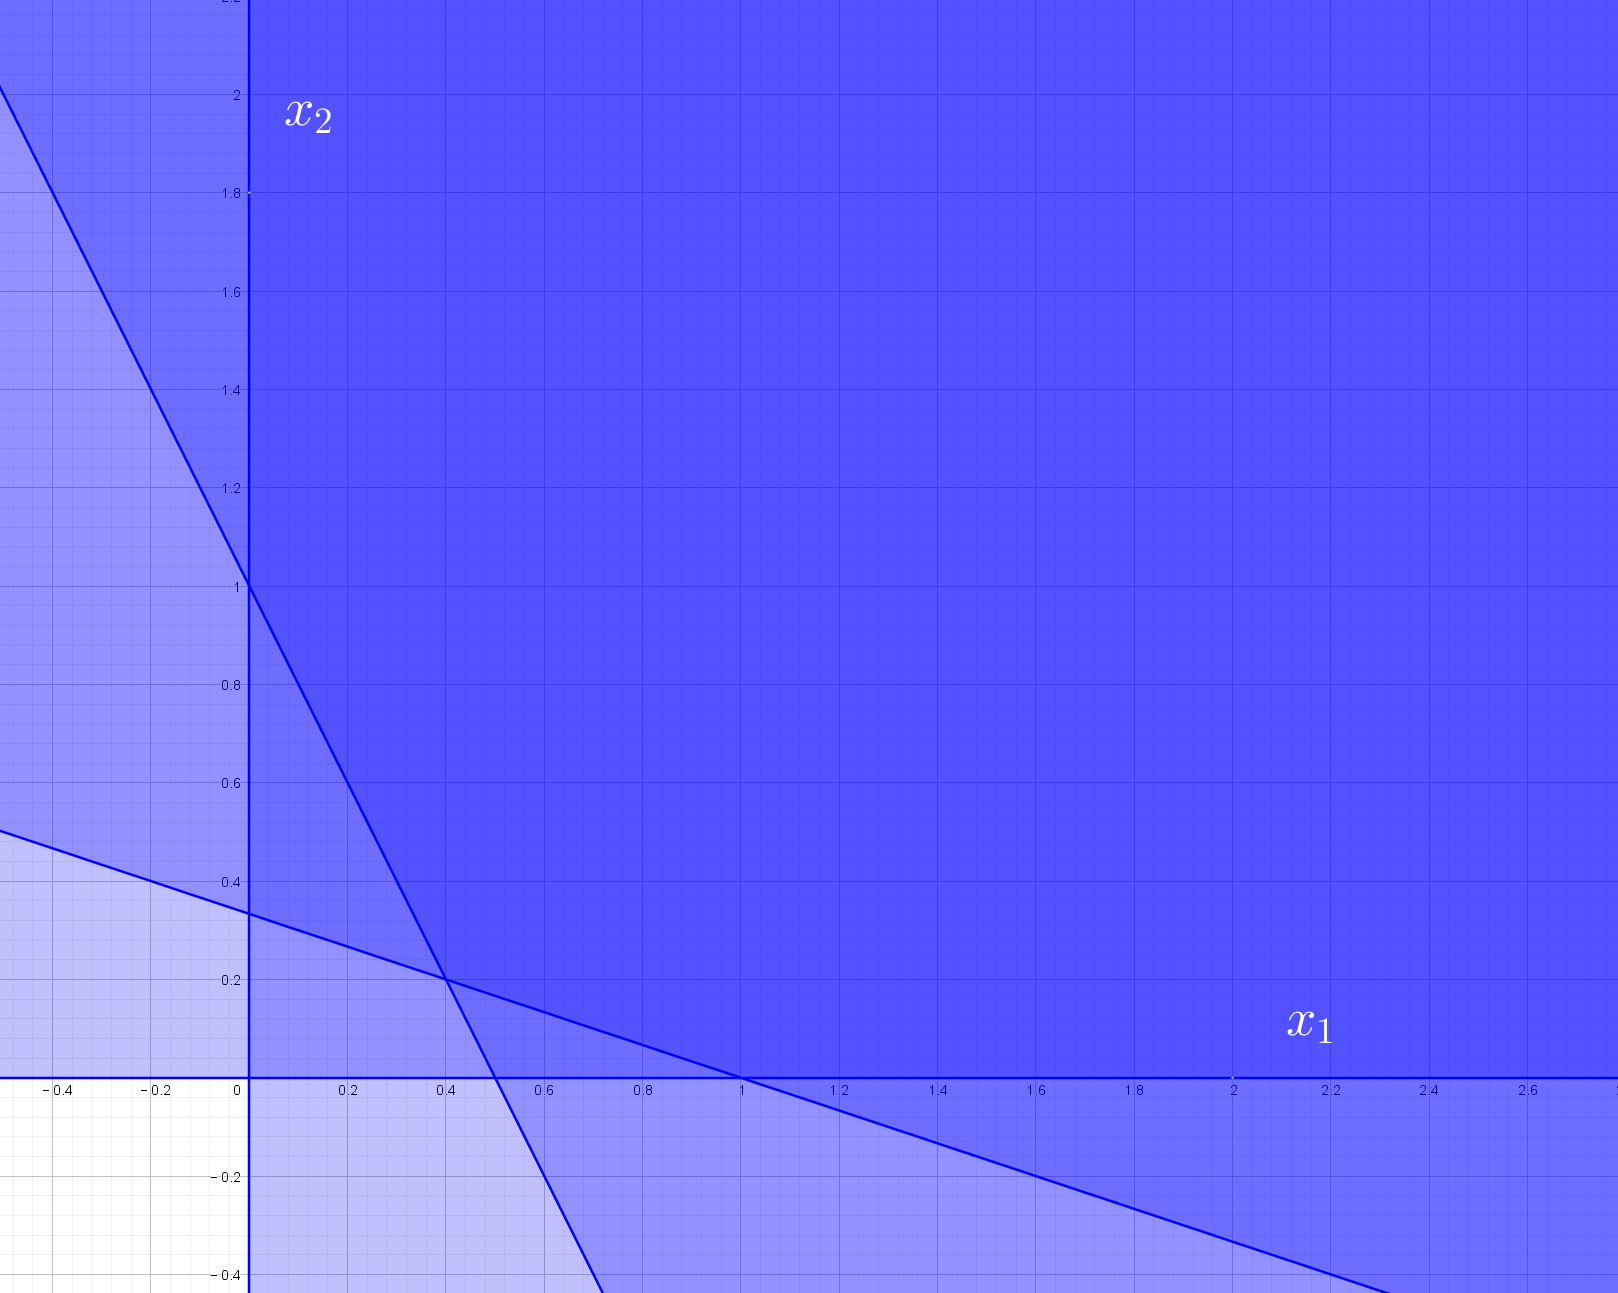
\includegraphics[scale=0.18]{p1.png}
    \caption{约束范围图}
\end{figure}

\begin{enumerate}[(a)]
    \item 利用数形结合的思路解答本问:
    令$x_{2}=-x_{1}+z$,其中$z$为变量。
    
    在二维空间中移动该直线,如图2所示
    \begin{figure}[H]
        \centering
        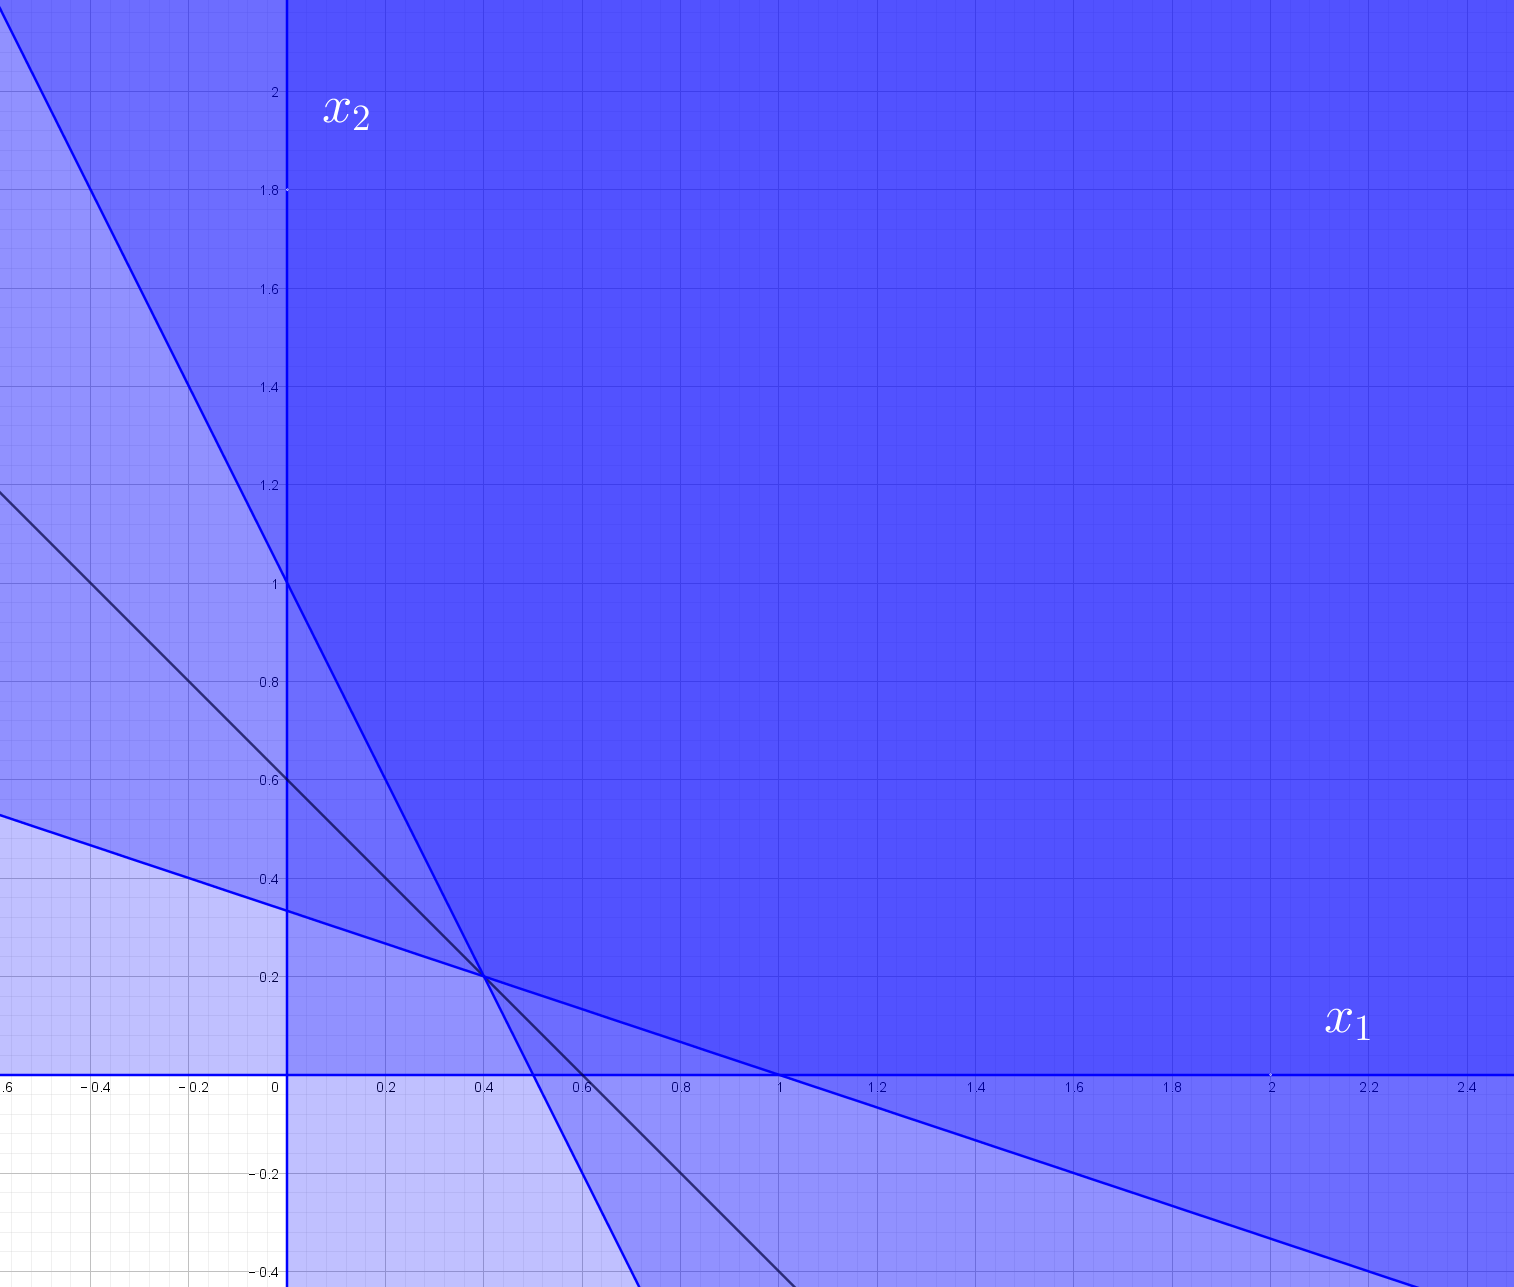
\includegraphics[scale=0.18]{p2.png}
        \caption{$x_{2}=-x_{1}+z$移动图}
    \end{figure}
    显然,当经过点$\left ( \frac{2}{5} ,\frac{1}{5}  \right ) $时,取得最优值。
    
    所以,$x^{*}= \left ( \frac{2}{5} ,\frac{1}{5}  \right ) $,最优值为$\frac{3}{5}$.

    \item 同(a)理,构造直线在二维空间中移动,如图3所示
    \begin{figure}[H]
        \centering
        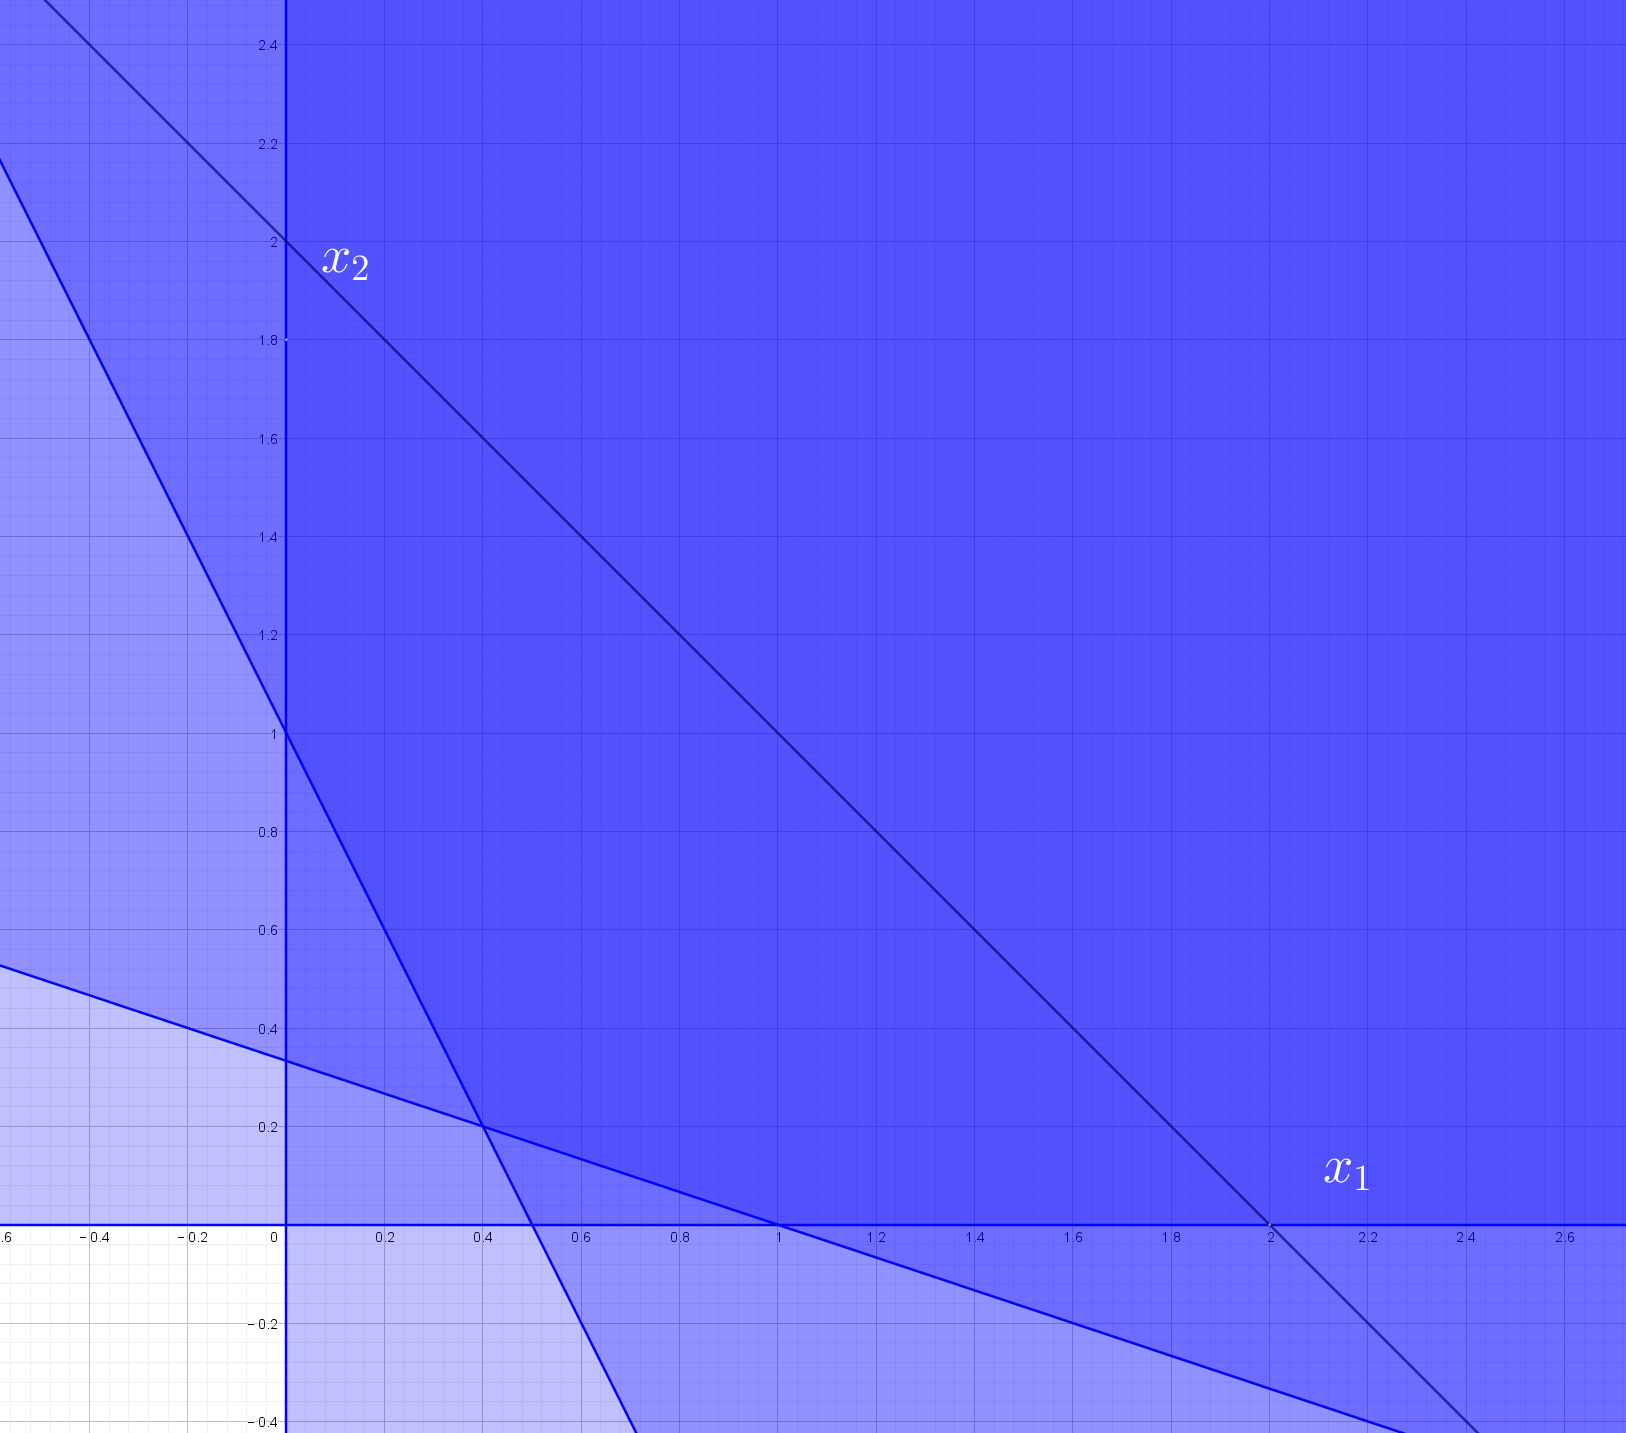
\includegraphics[scale=0.18]{p3.png}
        \caption{$x_{2}=-x_{1}-z$移动图}
    \end{figure}
    
    持续向上移动,$f_{0}\left(x_{1}, x_{2}\right)$均在可行集内,而$f_{0}\left(x_{1}, x_{2}\right)$的值逐渐减小。

    显然,$f_{0}\left(x_{1}, x_{2}\right)$无下界,因此最优值不存在。

    \item 最优值应满足$x_{1}=0$且$(0,x_{2})$在可行集内
    
    因此$x^{*}=\left\{\left(0, x_{2}\right) \mid x_{2} \geq 1\right\}$,最优值为0.

    \item 不妨设$x_{1} \ge x_{2}$,则问题可转化为如下形式:
    \begin{equation}
        \begin{array}{ll}
        \operatorname{minimize} & x_{1} \\
        \text {subject to} & 2 x_{1}+x_{2} \geq 1 \\
        & x_{1}+3 x_{2} \geq 1 \\
        & x_{1} \geq x_{2} \\
        & x \geq 0, \quad x_{2} \geq 0
        \end{array}
    \end{equation}
    做出该情况下的可行集如图4所示。
    \begin{figure}[H]
        \centering
        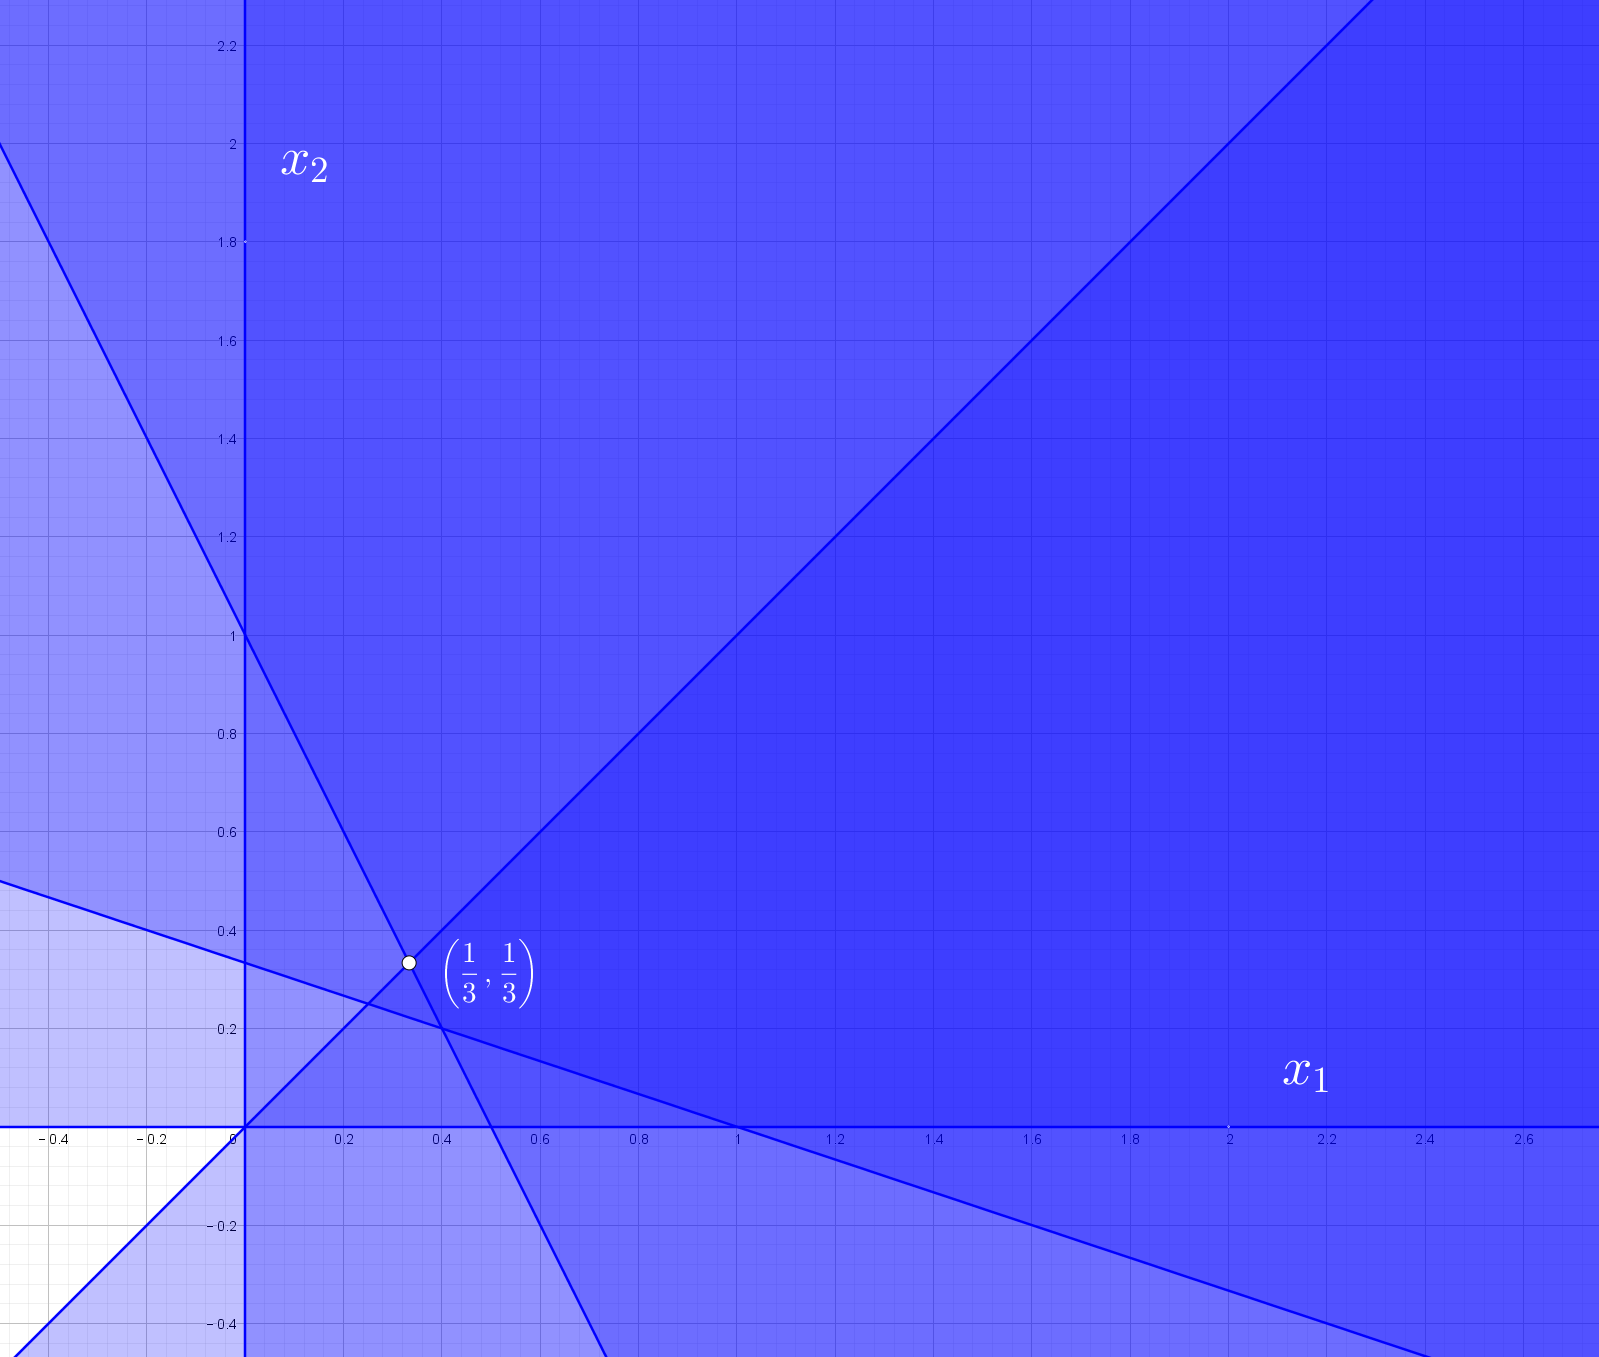
\includegraphics[scale=0.18]{p4.png}
        \caption{(1)式对应的可行集图}
    \end{figure}

    显然,$x^{*}= \left ( \frac{1}{3} ,\frac{1}{3}  \right ) $,最优值为$\frac{1}{3}$.

    讨论另一种情况,即$x_{1} \le x_{2}$时,问题可转化为如下形式:
    \begin{equation}
        \begin{array}{ll}
        \operatorname{minimize} & x_{1} \\
        \text {subject to} & 2 x_{1}+x_{2} \geq 1 \\
        & x_{1}+3 x_{2} \geq 1 \\
        & x_{1} \leq x_{2} \\
        & x \geq 0, \quad x_{2} \geq 0
        \end{array}
    \end{equation}
    做出该情况下的可行集如图5所示。
    \begin{figure}[H]
        \centering
        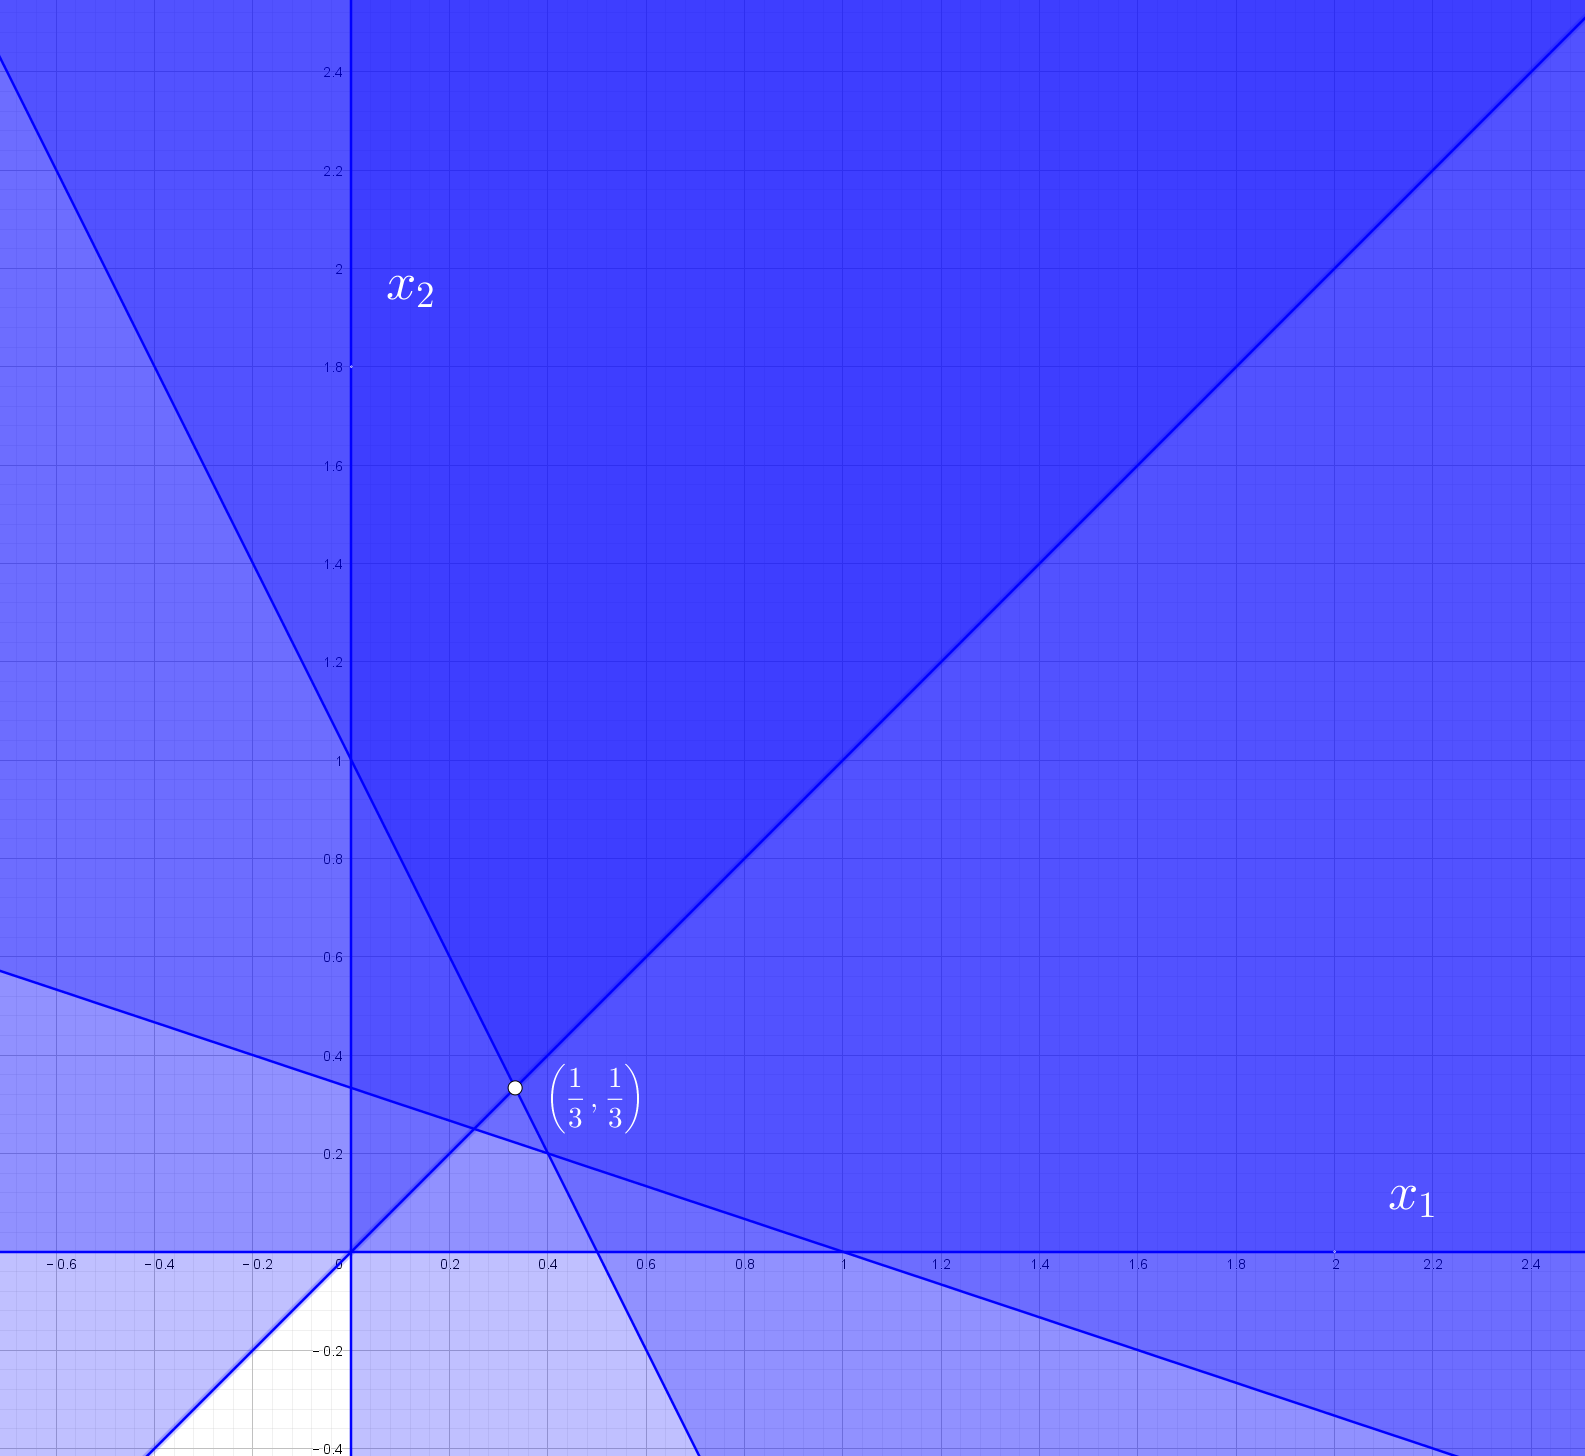
\includegraphics[scale=0.18]{p5.png}
        \caption{(2)式对应的可行集图}
    \end{figure}

    最优集与最优值与前一致。综上,$x^{*}= \left ( \frac{1}{3} ,\frac{1}{3}  \right ) $,最优值为$\frac{1}{3}$.

    \item 考虑KKT条件,
    
    \begin{eqnarray}
        \nabla_{\boldsymbol{x}} L(\boldsymbol{x}, \boldsymbol{\lambda}) = \mathbf{0} \Longrightarrow\left\{\begin{array}{l}
        2 x_{1}-2 \lambda_{1}-\lambda_{2} =0 \\
        18 x_{2}-\lambda_{1}-3 \lambda_{2}=0
        \end{array}\right.
    \end{eqnarray}

    假设$\lambda_{1}=0$,且$\nabla_{\boldsymbol{x}} L(\boldsymbol{x}, \boldsymbol{\lambda})=\mathbf{0}\,,\,\boldsymbol{\lambda}^{\top} \boldsymbol{g}(x)=\mathbf{0}$

    不难求得一组满足KTT条件的值为$x^{*}=(\frac{1}{2},\frac{1}{6})$,而$\left(\frac{1}{2}\right)^{2}+9 \cdot\left(\frac{1}{6}\right)^{2}=\frac{1}{2}$.

    因此,$x^{*}=(\frac{1}{2},\frac{1}{6})$,最优值为$\frac{1}{2}$.
\end{enumerate}
\end{document}

%%%%%%%%%%%%%%%%%%%%%%%%%%%%%%%%%%%%%%%%%%%%%%%%%%%%%%%%%%%%%%%%%%
%%%%%%%%%%%%%%%%%%%%%%%%%%%%%%%%%%%%%%%%%%%%%%%%%%%%%%%%%%%%%%%%%%
